
%(BEGIN_QUESTION)
% Copyright 2015, Tony R. Kuphaldt, released under the Creative Commons Attribution License (v 1.0)
% This means you may do almost anything with this work of mine, so long as you give me proper credit

Read and outline the ``Proximity Switches'' section of the ``Discrete Process Measurement'' chapter in your {\it Lessons In Industrial Instrumentation} textbook.  Note the page numbers where important illustrations, photographs, equations, tables, and other relevant details are found.  Prepare to thoughtfully discuss with your instructor and classmates the concepts and examples explored in this reading.

\underbar{file i04503}
%(END_QUESTION)





%(BEGIN_ANSWER)


%(END_ANSWER)





%(BEGIN_NOTES)

Proximity switches are non-contact position sensors.  Will be in its ``normal'' (resting) state when object is distant.  These are active devices, sensing objects using either inductance (metallic objects) or capacitance (non-metallic objects), or ultrasonic (dense objects).  Proximity switches often contain LED indicators to denote live status.

\vskip 10pt

Proximity switches are ``wet-contact'' devices, where they supply power to a load.  Sinking (NPN) switches connect load wire to negative side of power supply, while sourcing (PNP) switches connect load wire to positive side of power supply.  Sinking switches are sometimes referred to as ``low side'' devices, while sourcing switches are sometimes referred to as ``high side'' devices.

Standard color-codes for proximity switch wiring is:

\begin{itemize}
\item{} {\bf Brown} = (+) power supply
\item{} {\bf Blue} = ($-$) power supply
\item{} {\bf Black} = signal output
\end{itemize}

\vskip 10pt

Proximity switches come in normally-open as well as normally-closed forms.  This is unrelated to sinking vs. sourcing.  Switch characteristics such as sensing distance and ``normal'' status are often fixed at manufacture and not user-configurable.









\vskip 20pt \vbox{\hrule \hbox{\strut \vrule{} {\bf Suggestions for Socratic discussion} \vrule} \hrule}

\begin{itemize}
\item{} Identify some different designs of proximity switch.
\item{} How can we distinguish a proximity switch from a normal limit switch on a schematic diagram?
\item{} Identify the standard color-codes for electronic proximity switch wires.
\item{} Explain what the term ``dry contact'' refers to for a switch.
\item{} Explain what the terms ``normally open'' and ``normally closed'' refers to for a proximity switch.
\item{} Explain a procedure you could use for testing a proximity switch on a workbench using only a DC power source, a multimeter, and some alligator-clip style jumper wires.
\item{} Distinguish between ``low-side'' and ``high-side'' proximity switch types.
\item{} The application shown in the book where a proximity switch detects the motion of a link chain is one where a proximity switch is {\it definitely} superior to a direct-contact limit switch.  Explain why.
\end{itemize}














\vfil \eject

\noindent
{\bf Summary Quiz:}

Identify whether the proximity switch shown in this schematic diagram is a {\it sourcing} type or a {\it sinking} type:

$$\includegraphics[width=15.5cm]{i04503x01.eps}$$


\vfil \eject

\noindent
{\bf Summary Quiz:}

Identify whether the proximity switch shown in this schematic diagram is a {\it sourcing} type or a {\it sinking} type:

$$\includegraphics[width=15.5cm]{i04503x02.eps}$$

%INDEX% Reading assignment: Lessons In Industrial Instrumentation, proximity switches

%(END_NOTES)

